\documentclass[11pt]{article}
\usepackage{geometry} % see geometry.pdf on how to lay out the page. There's lots.
\usepackage{hyperref}
\usepackage{graphicx}
\usepackage{gensymb}
\usepackage[affil-it]{authblk}
\usepackage[toc,page]{appendix}
\usepackage{pifont}
\usepackage{amsmath}
\usepackage{float}
\usepackage{draftwatermark}

\SetWatermarkText{DRAFT}
\SetWatermarkScale{6}
\SetWatermarkLightness{0.95}

% \geometry{letter} % or letter or a5paper or ... etc
% \geometry{landscape} % rotated page geometry

% See the ``Article customise'' template for come common customisations

\title{The Design and Construction of a Novel Variable-Geometry Snake-like Input Device}

\author{Robert L. Read
  \thanks{read.robert@gmail.com}
  email: \href{mailto:read.robert@gmail.com}{read.robert@gmail.com}\\
Avinash Baskaran
  \thanks{baskaran.avinash@gmail.com}
  email: \href{mailto:Baskaran.avinash@gmail.com}{baskaran.avinash@gmail.com}
  }
  \affil{Public Invention, an educational non-profit.}


\date{\today}

%%% BEGIN DOCUMENT
\begin{document}

\maketitle

%% \tableofcontents

\begin{abstract}

	Humans are skillful. By building a bio-inspired manipulable snake-like controller that can be molded into a wide variety of shapes, we allow a human controller to telepresently specify complex shapes and shape changes. We constructed a tetrahelix consisting of seven tetrahedron made of adjustable-length members connected via 3D printed Song-Kwon-Kim joints which allow manual changes to the shape of the controller. These changes in length are digitized and organized via an Arduino and transmitted to more power computers where they may specify a shape to be animated or control a robot of similar shape, or simply specify relative positions in Cartesian space. Although this research is basic, we hope it will eventually amplify human control of in vivo mechanical devices such as endoscopes, search-and-rescue robots weaseling into tight spaces, or general purpose tetrobots used for planetary space exploration as suggested by Prof. Sanderson and his students 20 years ago.s

\end{abstract}


\section{Introduction}

Snake-like robots are particularly advantageous due to their ability to adopt varying geometries to navigate curvilinear paths.  They accomplish body undulation as a method of locomotion via . The design and construction of such objects relies on flexible actuation with respect to the field of motion.

  We have developed a biomimetically inspired hand-held input device, the motion of which can be digitally mapped onto the existing control mechansisms of robotic systems of to offer users and operators a direct human-robot interface for control. Snake-like robots are particularly advantageous due to their ability to adopt varying geometries to navigate curvilinear paths. Our device can be manipulated in 3-space to conform to various geometries such that the operation of linear robots in 3-space can be accomplished. As such, our device offers users a more organic movement control mechanism, which is highly favorable for applications where sensitive control and feedback are required. 

 As described in [Avinash1], Snake-like robots traditionally accomplish locomotion via body undulation using passive mechanisms to overcome environmental non-uniformities on 2-dimensional surfaces. Weight distribution mechansisms allow for undulation in the 3rd dimension, allowing  such robots to fully  mimic the mechanism of snakes. The control of snake-like robots often relies on static control mechanisms or digital path planning, while our controller is capable of being dynamically manipulated to accomplish these snake-like movements, and is thus a more favorable mechanism to operate snake-like robots.

 The simplistic design and construction of the device enables lightweight, modular deployment, with removeable components that allow for rapid repairs, and flexible design augmentation; the device design intrinsically encourages the addition of sensors, and end effector analogues upon its frame to control custom robotic implements, making it suitable for a variety of applications.


\subsection{Motivation}

While digital feedback and control mechanisms are useful due to their considerably greater reaction speed, high degree of autonomy, and dependable performance, there exist many applications in which human input is favorable. Our intuitive understanding of the locomotion we wish to accomplish in a given task and innate risk/reward analysis allows us to make decisions with a degree of creativity and complexity that is prohibitively high to provide in all circumstances. In such circumstances, providing a mechansim to translate human control allows for an integration of these aspects with existing control and feedback structures to optimize performance.
\section{Abstract Design}
\subsection{Tretrahelix}
\subsection{Linear Displacement to Cartesian}
\subsection{The \textit{Turret} Joint}

We employ a novel spherical joint designed by Song et. al. \cite{song2003spherical}, which serves as an effective method for joining linear sections in a tetrahedral configuration while allowing fixed and defined points of rotation. This joint offers a number of unique advantages that make it uniquely suited to our application; its rounded shape makes it an effective gripping tool for the human hand. The ability to alter the geometry of the hole, rotor and shell allows for customizable limits on the range of motion of the device. Most importantly, its removable, two part construction allows for easy addition or removal of single tetrahedra from the larger device, which in conjunction with the modularity of the tetrahedra, allows for a completely customizeable and arbitrary device.        
\subsection{Related Research}

\section{Method and Embodiment}
\subsection{Linear Potentiometers}
\subsection{3D Printred parts}
\subsection{Microelectronics}
 \begin{enumerate}
 \item Mechanism
 \item Housing
 \item Multiplexing
 \item Wireless communication
 \end{enumerate}

 The controller consists of an array of tetrahedrally arranged linear potentiometers embedded within 3D printed sleeve components, which comprise the device's physical framework. Each linear potentiometer allows for measurements of displacement along a single axis, which allows us to map the movement orientation of each sleeve simply using the analog output of each sensor. Each tetrahedron, groupings of 6 linear potentiometers, forming functional subdividisions of the structure, is provided a voltage input, ground, and signal output chanenel via onboard 8-channel multiplexers mounted to a single sleeve within the corresponding tetrahedron.

 [Discuss printed parts, mechanics and dynamics:]
 A controlled flexibility of an otherwise rigid the device,is provided by a spherical joint, invented by Song, Kwon, and Kim [?], depicted conceptually in (figure?: Song, Kwon, Kim, patent image) and (figure?: Turret Joint Planar Geometry).
 
\begin{figure}[H]
  \centering
    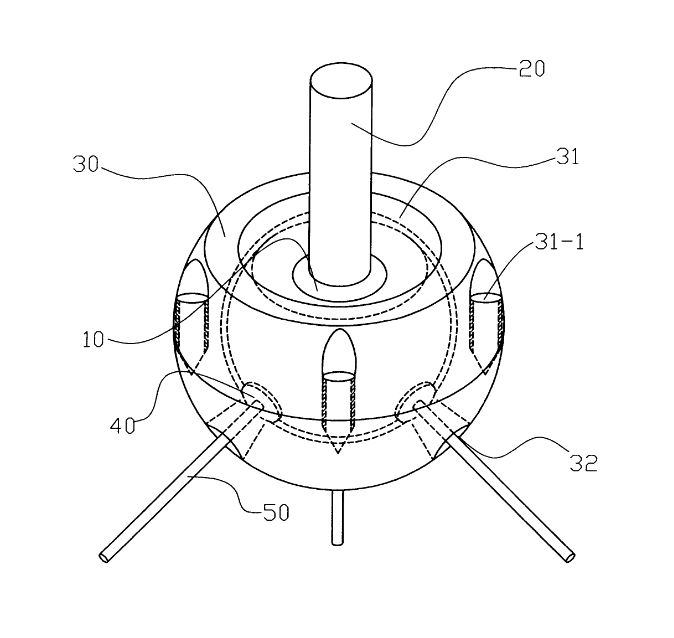
\includegraphics[width=0.5\textwidth]{figures/SongKwonKimImage.png}
    \caption[Song, Kwon, Kim, patent image.]{Song, Kwon, Kim, patent image.}
      \label{SongKwonKimImage}
\end{figure}


\begin{figure}[H]
  \centering
  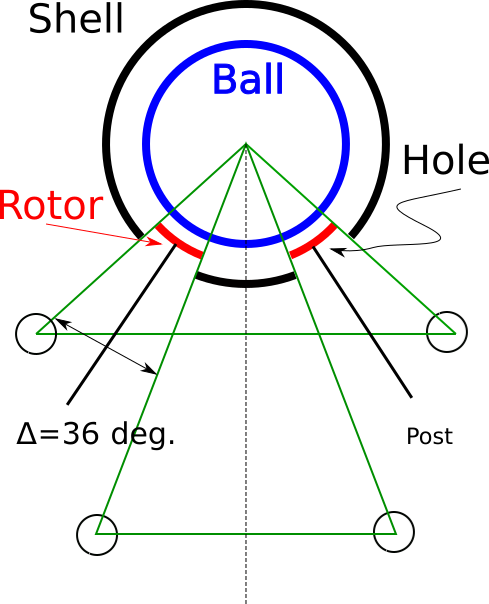
\includegraphics[width=0.5\textwidth]{figures/SimplifiedConstraintDrawing.png}
    \caption[Turret Joint Planar Geometry]{Turret Joint Planar Geometry}
      \label{simplified-constraint-drawing}
\end{figure}
 
 The  multiplexers send data from the (exact number?) sensors at near real-time to our processing unit, an Arduino Uno microcontroller, which provides 5V supply, ground, analog inputs, and digital control outputs to each of the multiplexers, and streams the data from each sensor via (bluetooth?) to an external location which can create a virtual reconstruction of the device, or further send data to a corresponding robot to be controlled. The use of multiplexers allows the singals from the potentiometers to be read together with little delay time between readings. The result of this system is the ability to precisely match the movement of the controller by a robot receiving the data. We have demonstrated this in (figure?: Screenshot of live visualization of the TetraCon using Dr. Read's software) and in (link?: video of Tetrobot being operated using TetroCon).
     
\subsection{System Design}
\section{Applications and Uses}
\subsection{Animation and Shaping}
\subsection{Medical Telepresence}

The human body, containing organ systems that are comprised of narrow fluidic channels, is a significant theater of operation for snake-like robots, both in surgical intervention and rehabilitation. Robotic implements used to treat and examine internal structures within human bodies often require manipulation and precise positioning by experienced professionals so as to not harm or injure the patient. Endoscopy instruments are often directly manipulated by hand, or remotely by computer-aided visual monitoring systems, however the difficulty in navigating such systems often results in undue pain to the patient due to impacts against channel walls. As a result of the limited range of motion and the intrinsic complexity of human organ systems, current mechanisms require more intuitive and organic control mechanisms to minimize injuries. Physically flexible controllers might allow for the navigation of winding channels within the human body with a greater degree of versatility and user input.

 In the context of rehabilation and external applications, a key benefit of the device is its hollow structure, meant to aid in its actuation but instead used to form around limbs and appendeges.In this way, the device can offer greater accuracy than traditional over-the-arm sensors in force and torque measurements while not impeding movement or blood flow by restrictively binding against the skin as do many rehabilitative exoskeletons. Once placed around a patient's limb, the device can be conformed to the shape of the limb and displacements in the sensors in response to various movements can be correlated to force and torque measurements to provide important feedback regarding the patient's musculoskeletal function.

 Telepresence robots in use in operating rooms where surgery by conventional methods is prohibitively expensive or dangerous allow operators to conduct procedures that would otherwise be impractical with simplicity and ease by positioning and manipulating end effectors with graphical user interfaces. Their complexity and versatility make them ideal partners for physicans and surgeons doing complicated surgical procedures without the instability, lack of precision and latency in response time inherent in the manipulation of surgical tools by human hands. The TetraCon can offer the advantage of being flexible enough to allow complex maneuvers to be conducted quickly, while still reducing the instability of direct human involvement by shifting its axis of orientation to accomodate rapid movements. 

\subsubsection{Extra-terrestrial robot manipulation}

The need for a more intuitive and organic telepresence operator in the field of extraterrestrial exploration is evident in the current state of such control mechanisms; Robotic arms mounted on orbiting structures are often operated by telepresence controllers with limited physical similarities to their counterparts. The presence of organic control in such mechanisms might signficantly reduce the lead-time necessary to train operators using these controllers and improve their versatility in the field. Further, the counterparts of such mechanisms could be made more agile in response to this development, where less lag between operation of a controller and a robot can be established by reducing the complexity of having to translate between 2 dimensional coordinate refernce frames of controllers to 3 dimensional reference frames of the controllee; if the robot being controlled is physically analogous to the controller, less effort is required to translate the movements of the controller to the robot.

Snake-like robots are highly advantages for extra-terrestrial navigation as well, given the non-uniform terrain that must be navigated on other planetary bodies. The TetraCon presents an advantage in this field in that it is already well-suited for the control and operaiton of such robots by the nature of its design. [examples:] 
\subsubsection{Tetrobot Telepresence Controller}

The Tetrobot, an initial concept proposed by... [pull from Rob's section] 
\section{Future Work}
\subsubsection{Reuse of current open-source code and models}
\subsubsection{Camera-based direct Cartesian Sensing}

END

///////////////////////////////////







Between 1996 and 2002 years ago, Arthur C. Sanderson and his colleagues published a series of
papers\cite{sanderson1996modular,lee2002dynamic,lee1999dynamics} on modular robots.
The ``TETROBOT'' was a variable-geometry truss, in which motion was accomplished by the change
in length of linear actuators, connected in a modular geometry based on the tetrahedron and octahedron.  Such a system
requires a special joint which allows the actuators to remain aimed at the center of joints while supporting
a certain amount of rotation about this center.


This paper builds upon that work by
introducing 3D-printable embodiments of
a recently invented spherical joint\cite{song2003spherical},
and gives some results related to the underlying geometry and math, as well as providing
references to all of the open-source materials needed to duplicate and expand on this work. This is an
open-source embodiment of the TETROBOT with physically smaller actuators which is more accessible to the
hobbyist or researcher with a limited budget.  The development of 3D printers, Bluetooth, microprocessors
such as the Arduino, and inexpensive commercial actuators has made this possible.
A very simple robot having only three tetrahedra is shown to be capable of locomotion.

\subsection{Motivation}

Imagine a strong, light, metamorphic material that can exert or resist force.
You can command it to form any shape, limited only by its flexibility.
Using that coformability you can get it to crawl across very rough terrain.
You can command it to form into a bridge or to lift and move heavy objects,
or to perform all the functions of a crane, a forklift, a backhoe and/or bulldozer.

\begin{figure}[H]
  \centering
    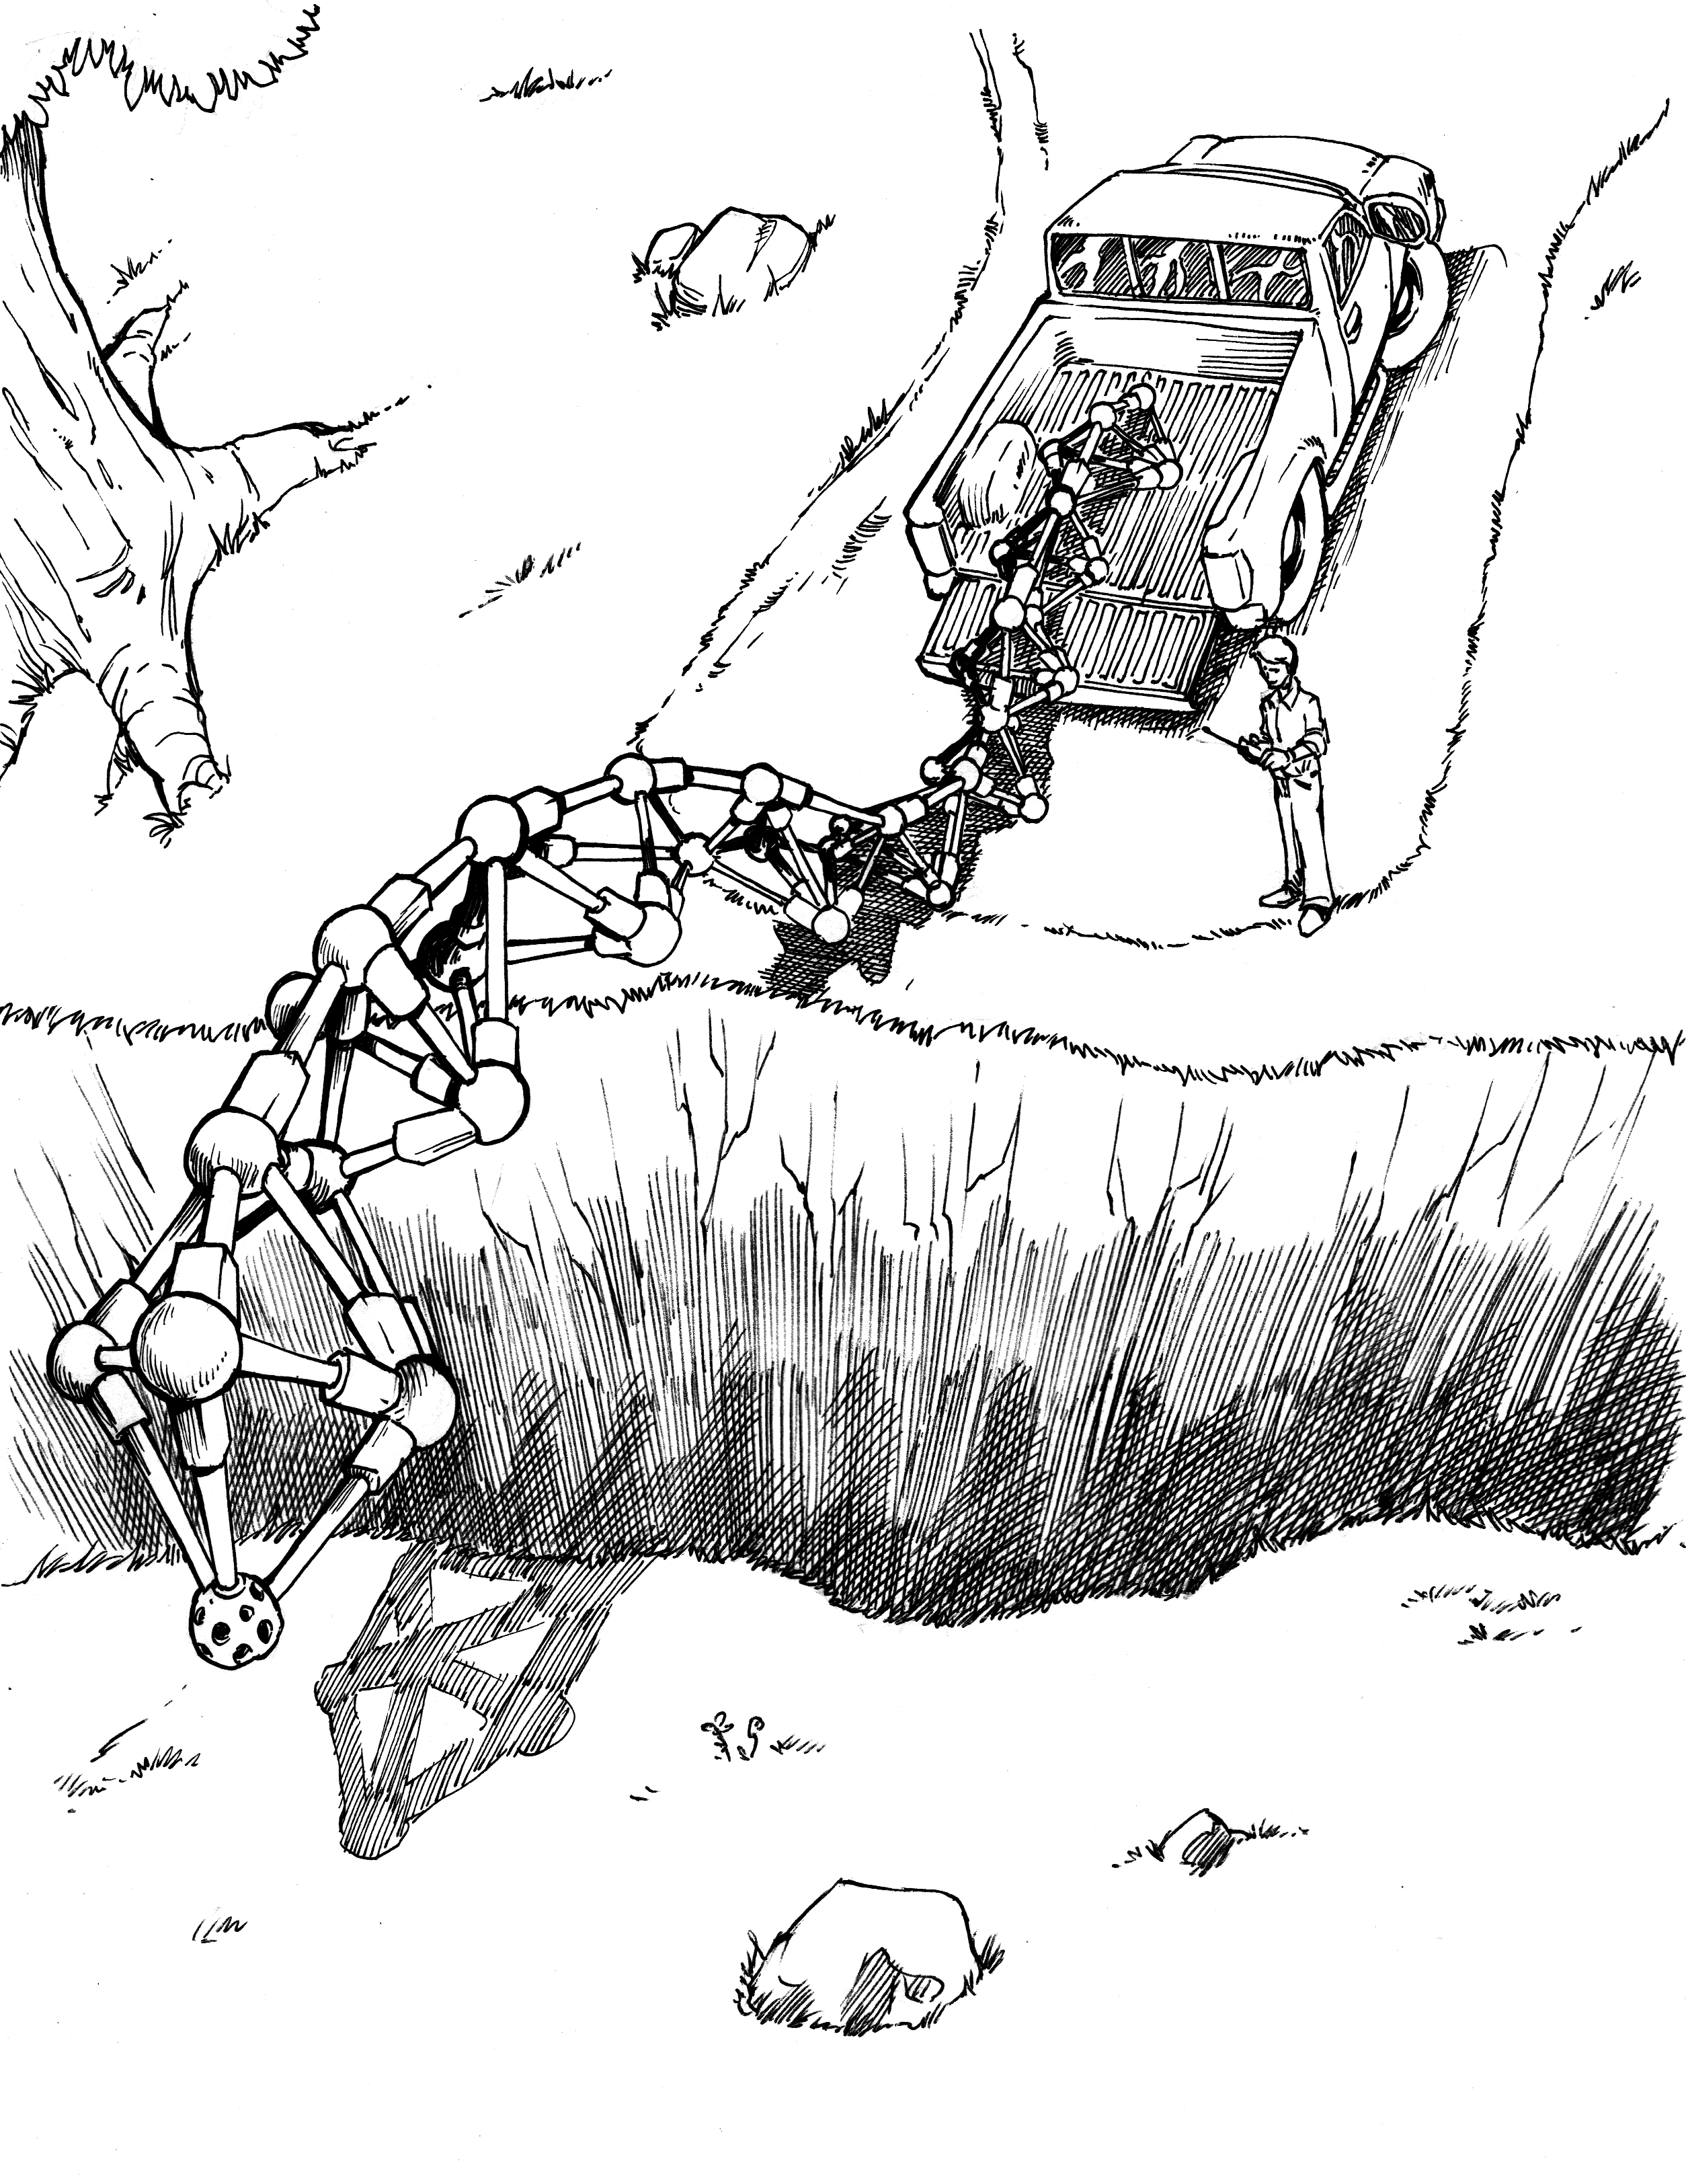
\includegraphics[width=0.5\textwidth]{figures/robotTruckChasm.png}
    \caption[Concept art of GlussBot Spanning a Chasm]{Concept art of GlussBot Spanning a Chasm}
      \label{chasmspan}
\end{figure}

It is a truss that crawls like a slug---a \emph{gluss}.
If you need more of it, you buy it by the kilo and when it arrives you order it
to crawl to your existing gluss. You easily join it there, creating
larger, stronger, combined mass.

The advantages of snakebots have been widely recognized %%\cite{liljebäck2012snake}.
In general, these have been constructed
with angular joints. In this paper we propose a different, truss-like approach to providing similar
mobility that uses only linear actuators and spherical joints that eliminates non-axial forces so that only
compressive and tensile forces act on the actuators.
This potentially combines the advantages of forceful machines with snake-like mobility.


Other geometries, such as moving planes, are possible with the same material.

Additional videos at the YouTube channel, Public Invention, reachable from the above link,
further motivate the \emph{gluss} concept.

\subsection{Concept: Gluss = Slug + Truss}

Imagine a metamorphic or polymorphic machine that forcefully assumes a variety of shapes. It moves like a mollusc or amoeba,
oozing into position as commanded. It is technically a ``machine'' because it can exert force reliably, but
it may be thought of as a material, because unlike most robots its components are not differentiated.

Although someday an actual chemical substance may do this, today it can be constructed from commercial components
and 3D-printable parts. This paper introduces the \emph{gluss} approach to building metamorphic dynamic robots
and static machines.\footnote{ ``Gluss'' is a portmanteau of ``Slug'' and ``Truss'' because we are attempting to
build a truss, or space frame, that is capable of moving like a slug or octopus.
The word \textit{gluss}
should be used as a substantive noun in English, much like the word \textit{clay} is used.
The use of \textit{glusses}, the plural
of \textit{gluss}, should be rare and refer to different kinds of metamorphic material, such as the expression
``four clays'' suggests four distinct types of clay without specifying how many kilograms of each one means.}

Massively scalable robots have often been proposed. Our particular approach is to use linear actuators,
which are rod-like machines that can make themselves shorter or longer. These are tied together using
a relatively new joint \cite{song2003spherical} which allows, for example, as many as 12, but more realistically 4 or 6,
members to be joined together sturdily at a single point.
A 3-D printed embodiment presented here, called the \emph{turret joint}, allows the
change of angle required for the gluss to ooze about. Some gluss consists of some actuators joined together
with some turret joints and whatever batteries and control microelectronics are needed.

\begin{enumerate}
\item Design concept
\item Control:
  \begin{enumerate}
  \item Sensors
    \begin{enumerate}
    \item Mechanism
    \item Housing
    \item Wiring
    \item Circuit analysis (needed?)
    \end{enumerate}
  \item Signals
    \begin{enumerate}
    \item Multiplexing
    \item Wireless communication
    \end{enumerate}
  \end{enumerate}

\item Turret joint
  \begin{enumerate}
  \item Gluss-con scaling/proportions to the Gluss
  \item Universal joint / modularity
  \end{enumerate}
m\item Sleeves
  \begin{enumerate}
  \item Modularity
  \end{enumerate}

\item User-friendliness
  \begin{enumerate}
  \item … (experimentation?)
  \end{enumerate}
\item Applications
  \begin{enumerate}
  \item Assistive
    \begin{enumerate}
    \item Body-attached assistive / tertiary limb device
    \item Pole mounted arm
    \item Physically independent device
    \end{enumerate}
  \item Medical
    \begin{enumerate}
    \item Rehabilitation
      \begin{enumerate}
      \item Motor skill development for learning imparied children
      \item Skeleto-muscular rehab
      \item Physiotherapy
      \end{enumerate}
    \item Prosthetics / limb replacement
    \item Medical casts / sleeves
    \item Surgical assistant device
    \end{enumerate}
  \item Future work
    \begin{enumerate}
    \item Optical sensing
      \begin{enumerate}
      \item Computer - vision based detection
      \end{enumerate}
    \end{enumerate}
  \end{enumerate}
\end{enumerate}

\section{The \textit{Turret Joint}}

\subsection{The Need}

The way to make something large, light, and strong is to make it inherently rigid by building it
out of triangles. In a single plane, this is called a \emph{truss} \cite{ambrose1993building}, and more generally is called
a \emph{space frame}.  Space frames made completely from triangles tend to be rigid even if the
joints that connect members allow motion, such as a pin joint or a ball-and-socket joint. This
is an advantage because non-axial strain (that is, a slight change in the angular geometry of the frame)
cannot cause
the joint to fail, as it can with a welded joint.

But we seek a space frame that can change its shape dramatically. Imagine a radio tower in which
each girder has been replaced with an actuator that can get longer or shorter. Such a tower could
bend its top down to the ground, or even
tie itself into a knot. To accomplish this, the joints must support significant
but limited range of angular motion.

The spherical joint invented by Song, Kwon and Kim \cite{song2003spherical} is such a joint,
the essence of which is rendered in their patent drawing, Figure \ref{SongKwonKimImage}.
We name this joint the \emph{Turret Joint}.

\begin{figure}[H]
  \centering
    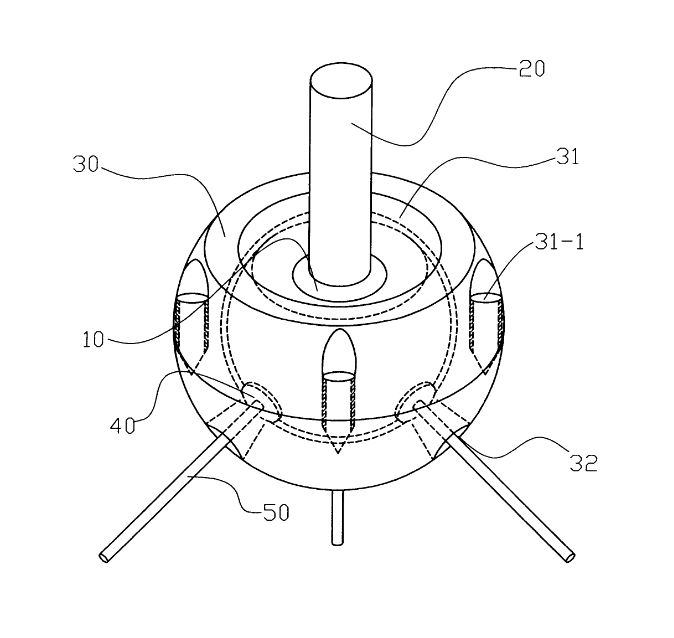
\includegraphics[width=0.5\textwidth]{figures/SongKwonKimImage.png}
    \caption[Song, Kwon, Kim, patent image.]{Song, Kwon, Kim, patent image.}
      \label{SongKwonKimImage}
\end{figure}

When properly configured to support regular nets of actuators,
it allows the gluss to be a moving space frame. It happens that the specific actuators we use
are geared such that when no power is applied, they strongly resist outside forces that would change their length,
essentially becoming rigid members.
The resulting gluss
can move into position and then be powered off to be a temporarily static space frame.

One could also use this joint with members which are not actuators. For example, we first
constructed the joint with carbon fiber rods. In essence it is then a construction kit with continuously
variable member lengths liberated from using a finite set of angles.

\subsection{Geometry}

\begin{figure}[H]
  \centering
  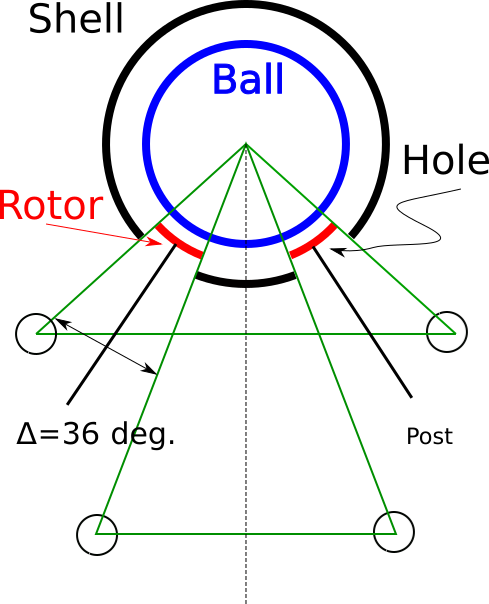
\includegraphics[width=0.5\textwidth]{figures/SimplifiedConstraintDrawing.png}
    \caption[Turret Joint Planar Geometry]{Turret Joint Planar Geometry}
      \label{simplified-constraint-drawing}
\end{figure}

One way to approach this problem is to consider a single triangle formed by joints and actuators.
The joint must support the most acute triangle
that can be formed with the three actuators and the most obtuse triangle that can be formed with the actuators.

In fact it is a surprising result that we prove elsewhere \cite{readglussbot} in Appendix A that the maximum $Q$ which can be utilized
by an ideal turret joint happens to be
the famous golden ratio, $\varphi \equiv \frac{1 + \sqrt{5}}{2} \approx 1.618...$, and the maximum deviation for any one member coming
into the joint is $36\degree$.
Thus in Figure \ref{simplified-constraint-drawing} the triangles drawn are in fact a Golden Triangle and a Golden Gnomon.
A real-world joint, which will support less variation because the ``post'' must have a
certain thickness and the ``rotor'' must have a lip
slightly larger than the hole in order to remain locked in place.
Furthermore, the joint adds a certain necessary thickness, the minimum length
 from joint-center to joint-center will be somewhat greater than from actuator tip to actuator tip.

 However, the theoretical ideal result is a valuable approach to physical computation and makes a $Q$ for a physical actuator of 1.5 seem quite appropriate.

 \subsection{Embodiment}

 Although the joint could be machined or formed in some other way,
 3D Printers have made the construction of the Turret Joint far easier.
 We have designed a complete set of components needed to 3D print the joint and the rotors to attach to
 the linear actuators. These models are created with OpenSCAD, a functional parametric modeling program.

 Our experience has been that the common plastics PLA and ABS are adequate for the Turret Joint,
 but have found that nylon, which is far tougher and less prone to cracking, is superior for the
 rotors which bolt directly to the actuators.

 \begin{figure}[H]
  \centering
    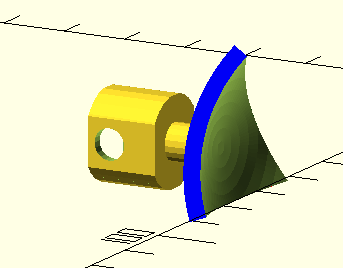
\includegraphics[width=0.5\textwidth]{figures/RotorModel.png}
    \caption[Triangular Rotor Model]{Triangular Rotor Model.}
      \label{rotormodel}
\end{figure}

 We have innovated the design of the rotor by using a triangular section of a sphere as the
 rotor rather than a circular section, as shown in Figure \ref{rotormodel}.
 Assuming that each actuator is free to rotate about its axis as well as revolve about the
 center of the ball joint, this shape does not limit motion even in the most pinched
 configurations. The triangular rotor provides greater extent of contact,
 which presumably makes the joint motion
 smoother and less likely to bind.


 The Figure below shows most of the parts. The nylon triangular rotor is white and rests upon
 the red ball. The green part is a Tetrahelix lock, and the yellow parts are the locks for the Octet Truss
 geometry.

\begin{figure}[H]
  \centering
    \includegraphics[width=0.7\textwidth]{figures/Parts.jpg}
    \caption[3D Printed Parts]{3D Printed Parts}
\end{figure}



\subsection{Open Source Realizations}

\section{Related Research}

Between 1996 and 2002, Arthur C. Sanderson and his colleagues published a series of
papers\cite{sanderson1996modular,lee2002dynamic,lee1999dynamics} on modular robots.
The ``TETROBOT'' was a variable-geometry truss, in which motion was accomplished but the change
in length of linear actuators, connected in a modular geometry based on the tetrahedron and octahedron.
A quadrupedal robot was constructed completely out of the tetrahedral/octahedral geometry.
The TETROBOT robots successfully walked and even rolled. The TETROBOT hardware was significantly
heavier and more powerful that then hardware used here. The glussbots have so far demonstrated no greater functionality,
although we have demonstrated that very simple robots consisting of only 3 tetrahedra can locomote.

The technology presented in this article has drastically lowered the cost,
thus making the glussbot/TETROBOT concept
accessible to hobbyists and researchers on a limited budget.

The TETROBOT used a joint called the CMS joint. Although
possibly superior in not allowing an extra degree or rotational freedom, it would be a challenge to use the CMS
joint with the Actuonix actuators because the pushrod must fully retract, or the length of the pushrod would be
have to be extended with an attachment. Sanderson's students used actuators that
extended from the middle, avoiding this problem. If the Gluss Project ever develops its own actuators, it should
explore using this joint.

If you read the introduction of the brilliant book by Shigoe Hirose\cite{hirose1993biologically} substituting
``even simpler soft squiggly thing that might not be as cylindrical as a snake'' for the word ``snake'', you will have
an excellent motivation for the gluss concept.  More generally, much of the work developed for snakebot
locomotion %%\cite{liljebäck2012snake}
is directly reusable, in the sense that a long enough tetrahelix can
model a snake, and further inspires the idea of using simpler models mapped into a gluss model to perform
complex movements.

Buckminster Fuller also promoted \emph{tensegrity}, and some research on Tensegrity Robots has been done, the
work of Paul, Valero-Cuevas, and Lipson\cite{paul2006} being a good starting point.
This work has developed into a serious effort\cite{NTRT} by NASA to explore tensegrity robots for extraterrestrial
exploration.

Tensegrities are closely related to the gluss concept, more researched, and potentially more performant.
In fact a gluss could be considered a special case of a tensegrity, using vanishingly short cables
and, in the terminology of \cite{paul2006}, \emph{strut-collocated actuation}.
It has been reasonable to produce a static gait for the 3TetGlussBot and 5TetGlussBot because its behavior is not
very dynamic: it is so slow and strong that velocity is irrelevant at the current scale.
Reported tensegrity robots have focused on dynamic, ``hopping'' and rolling gaits.

It is possible that gluss is easier to work with for an actual human being on the ground.
Although of course both systems will use computer control systems, one can imagine a large robot
crawling into place imperfectly, and some workperson making a manual adjustment: ``Actuator \#37, get shorter!''
This is intellectually more difficult for a tensegrity, wherein changing a cable length
has less predictable impact on the tensegrity geometry.
However, many
of the future steps outlined in Section \ref{futuresteps} apply to both gluss and tensegrity robots.

This paper presents the gluss as a ``machine'', rather than a ``mechanism''. That is, it motivates gluss
by asserting it can exert and resist force, yet currently treats gluss positioning as a purely kinematic,
rather than dynamic problem. The actuators currently in use are geared such that they are so slow
and powerful that the behavior is not really dynamic. If static analysis of a resulting geometry is
needed, for example to ask if structure used as a bridge will bear a load, a finite element approach\cite{geradin2001flexible}
will be adequate.

If one chooses to attempt to exert a high enough force or to move more quickly, classic robot control theory
which models forces and velocities based on Lagrangian mechanics will be required.

\section{Placeholder for Photos}

\begin{figure}[H]
  \centering
    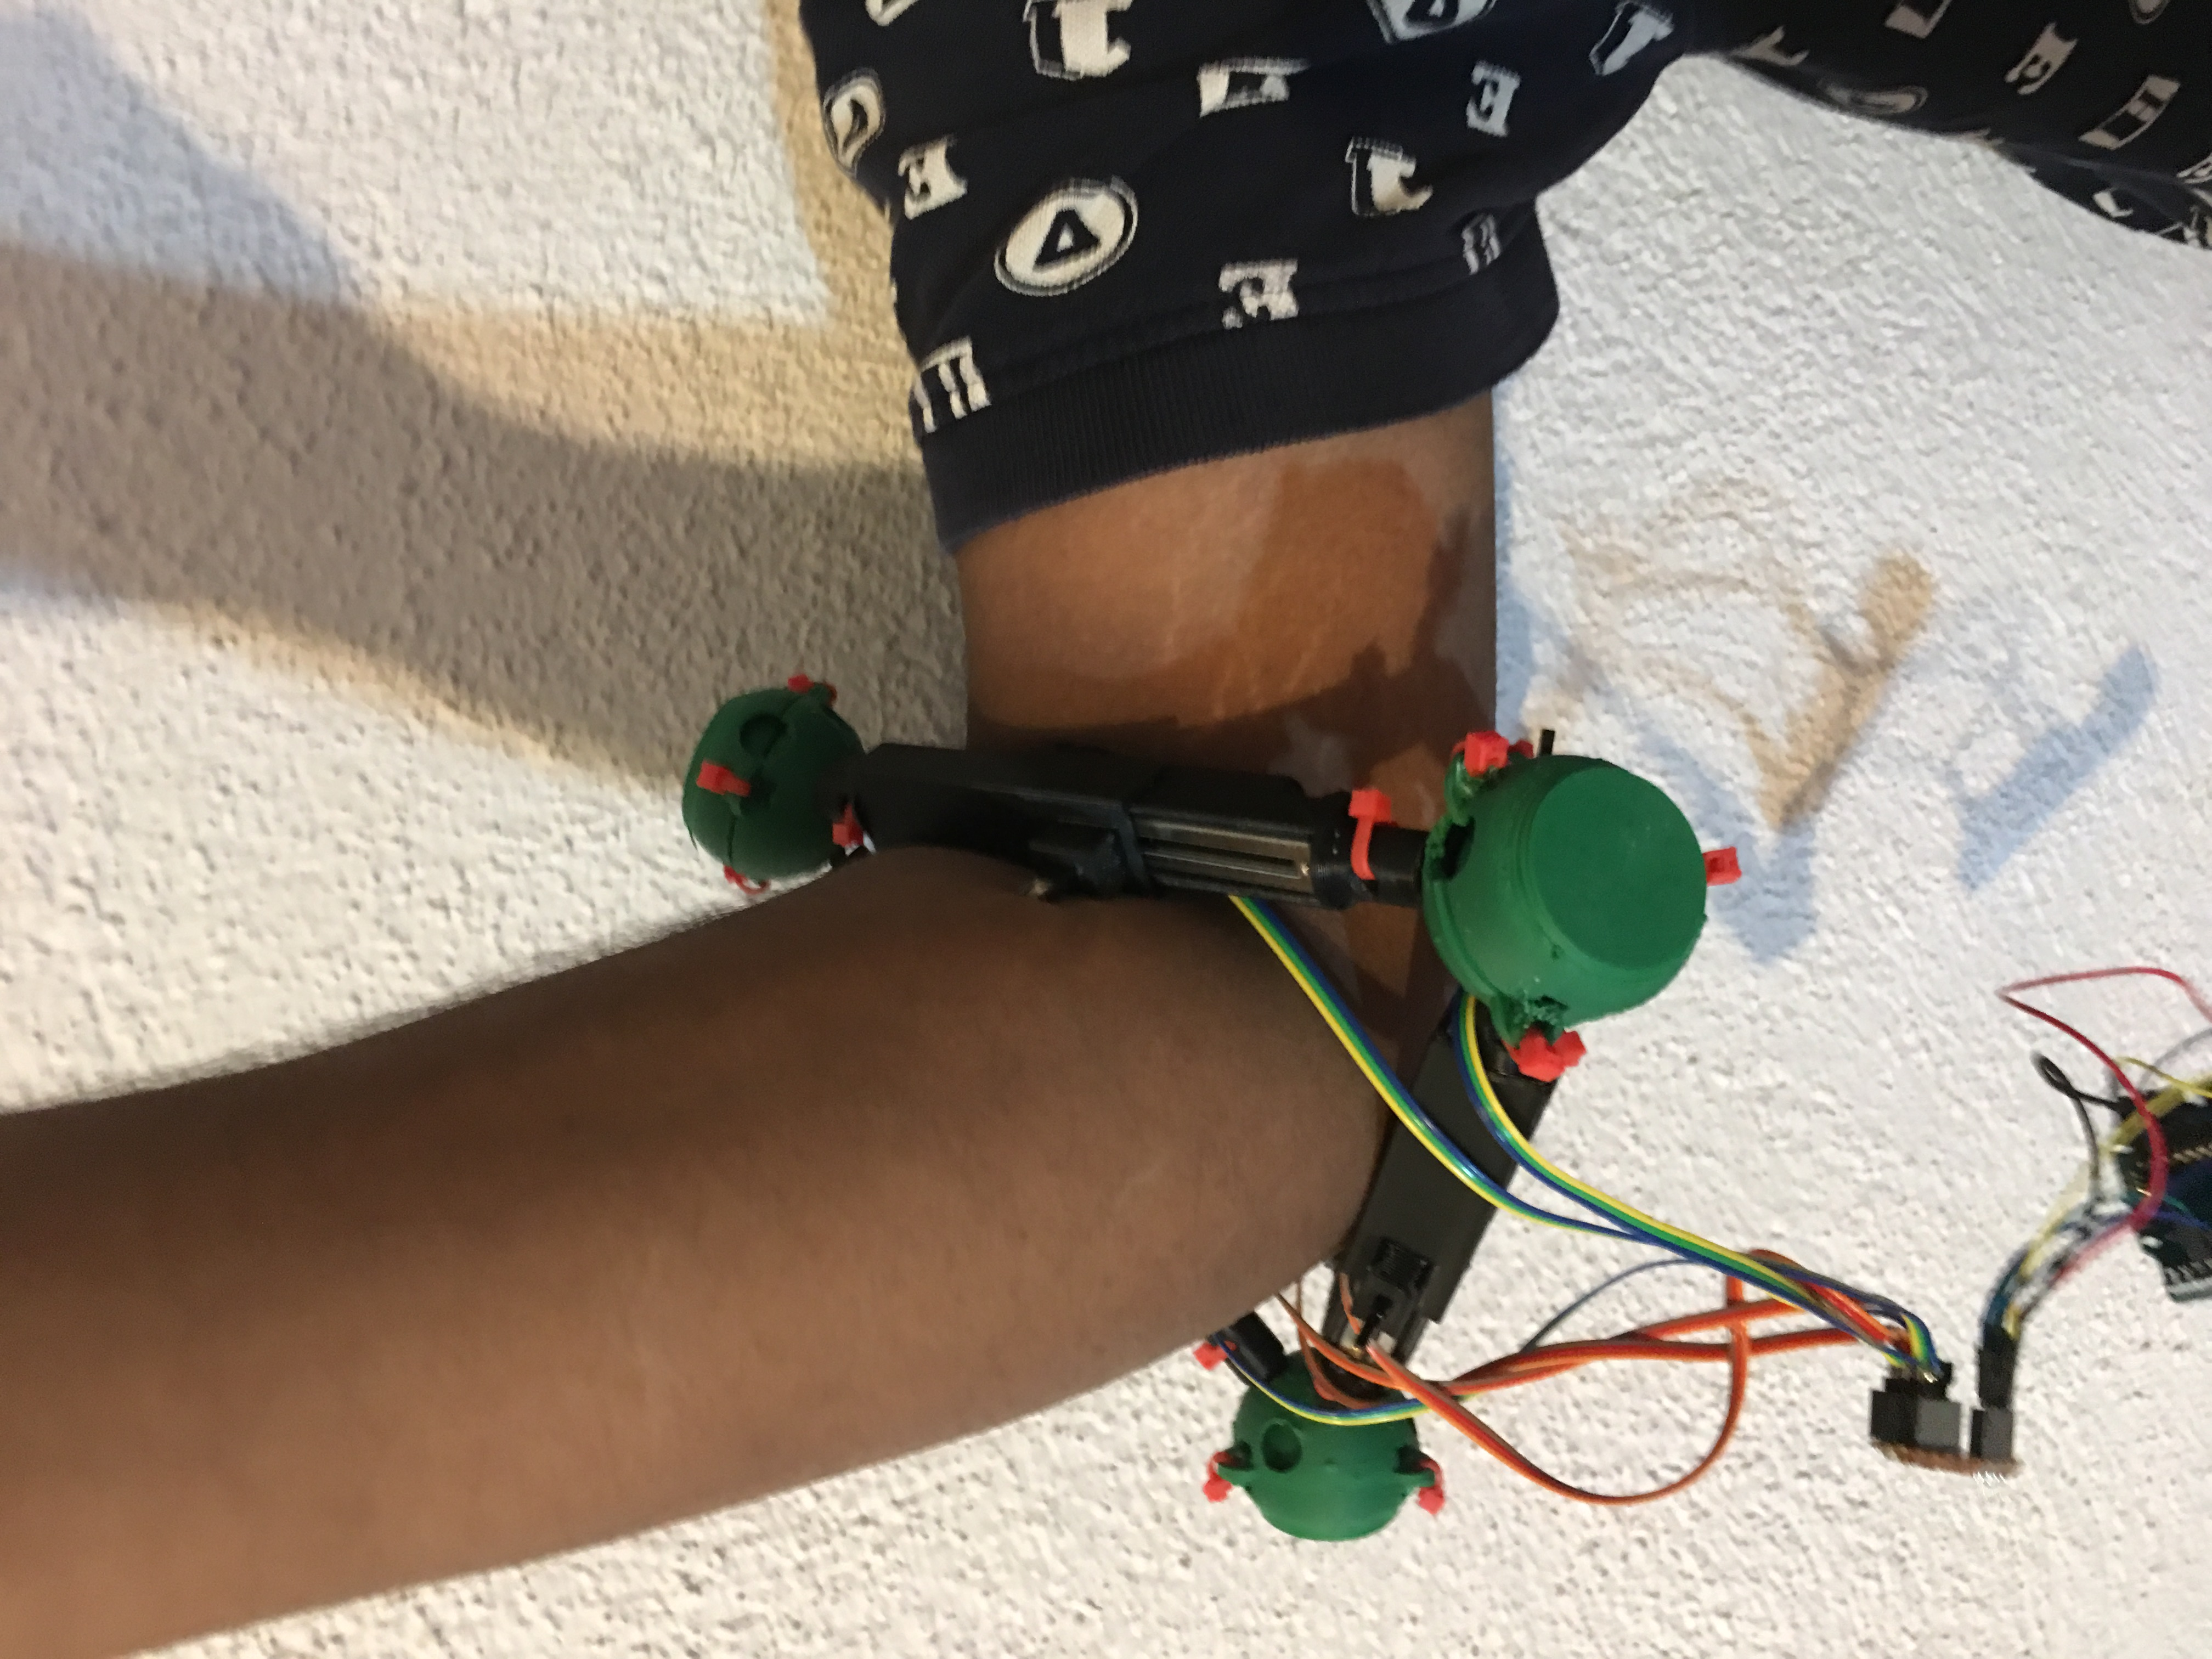
\includegraphics[angle=270,width=0.5\textwidth]{figures/ElbowFitting.JPG}
    \caption[One-tet controller fitting an elbow]{One-tet controller fitting an elbow}
      \label{fig:elbowfitting}
\end{figure}

\begin{figure}[H]
  \centering
    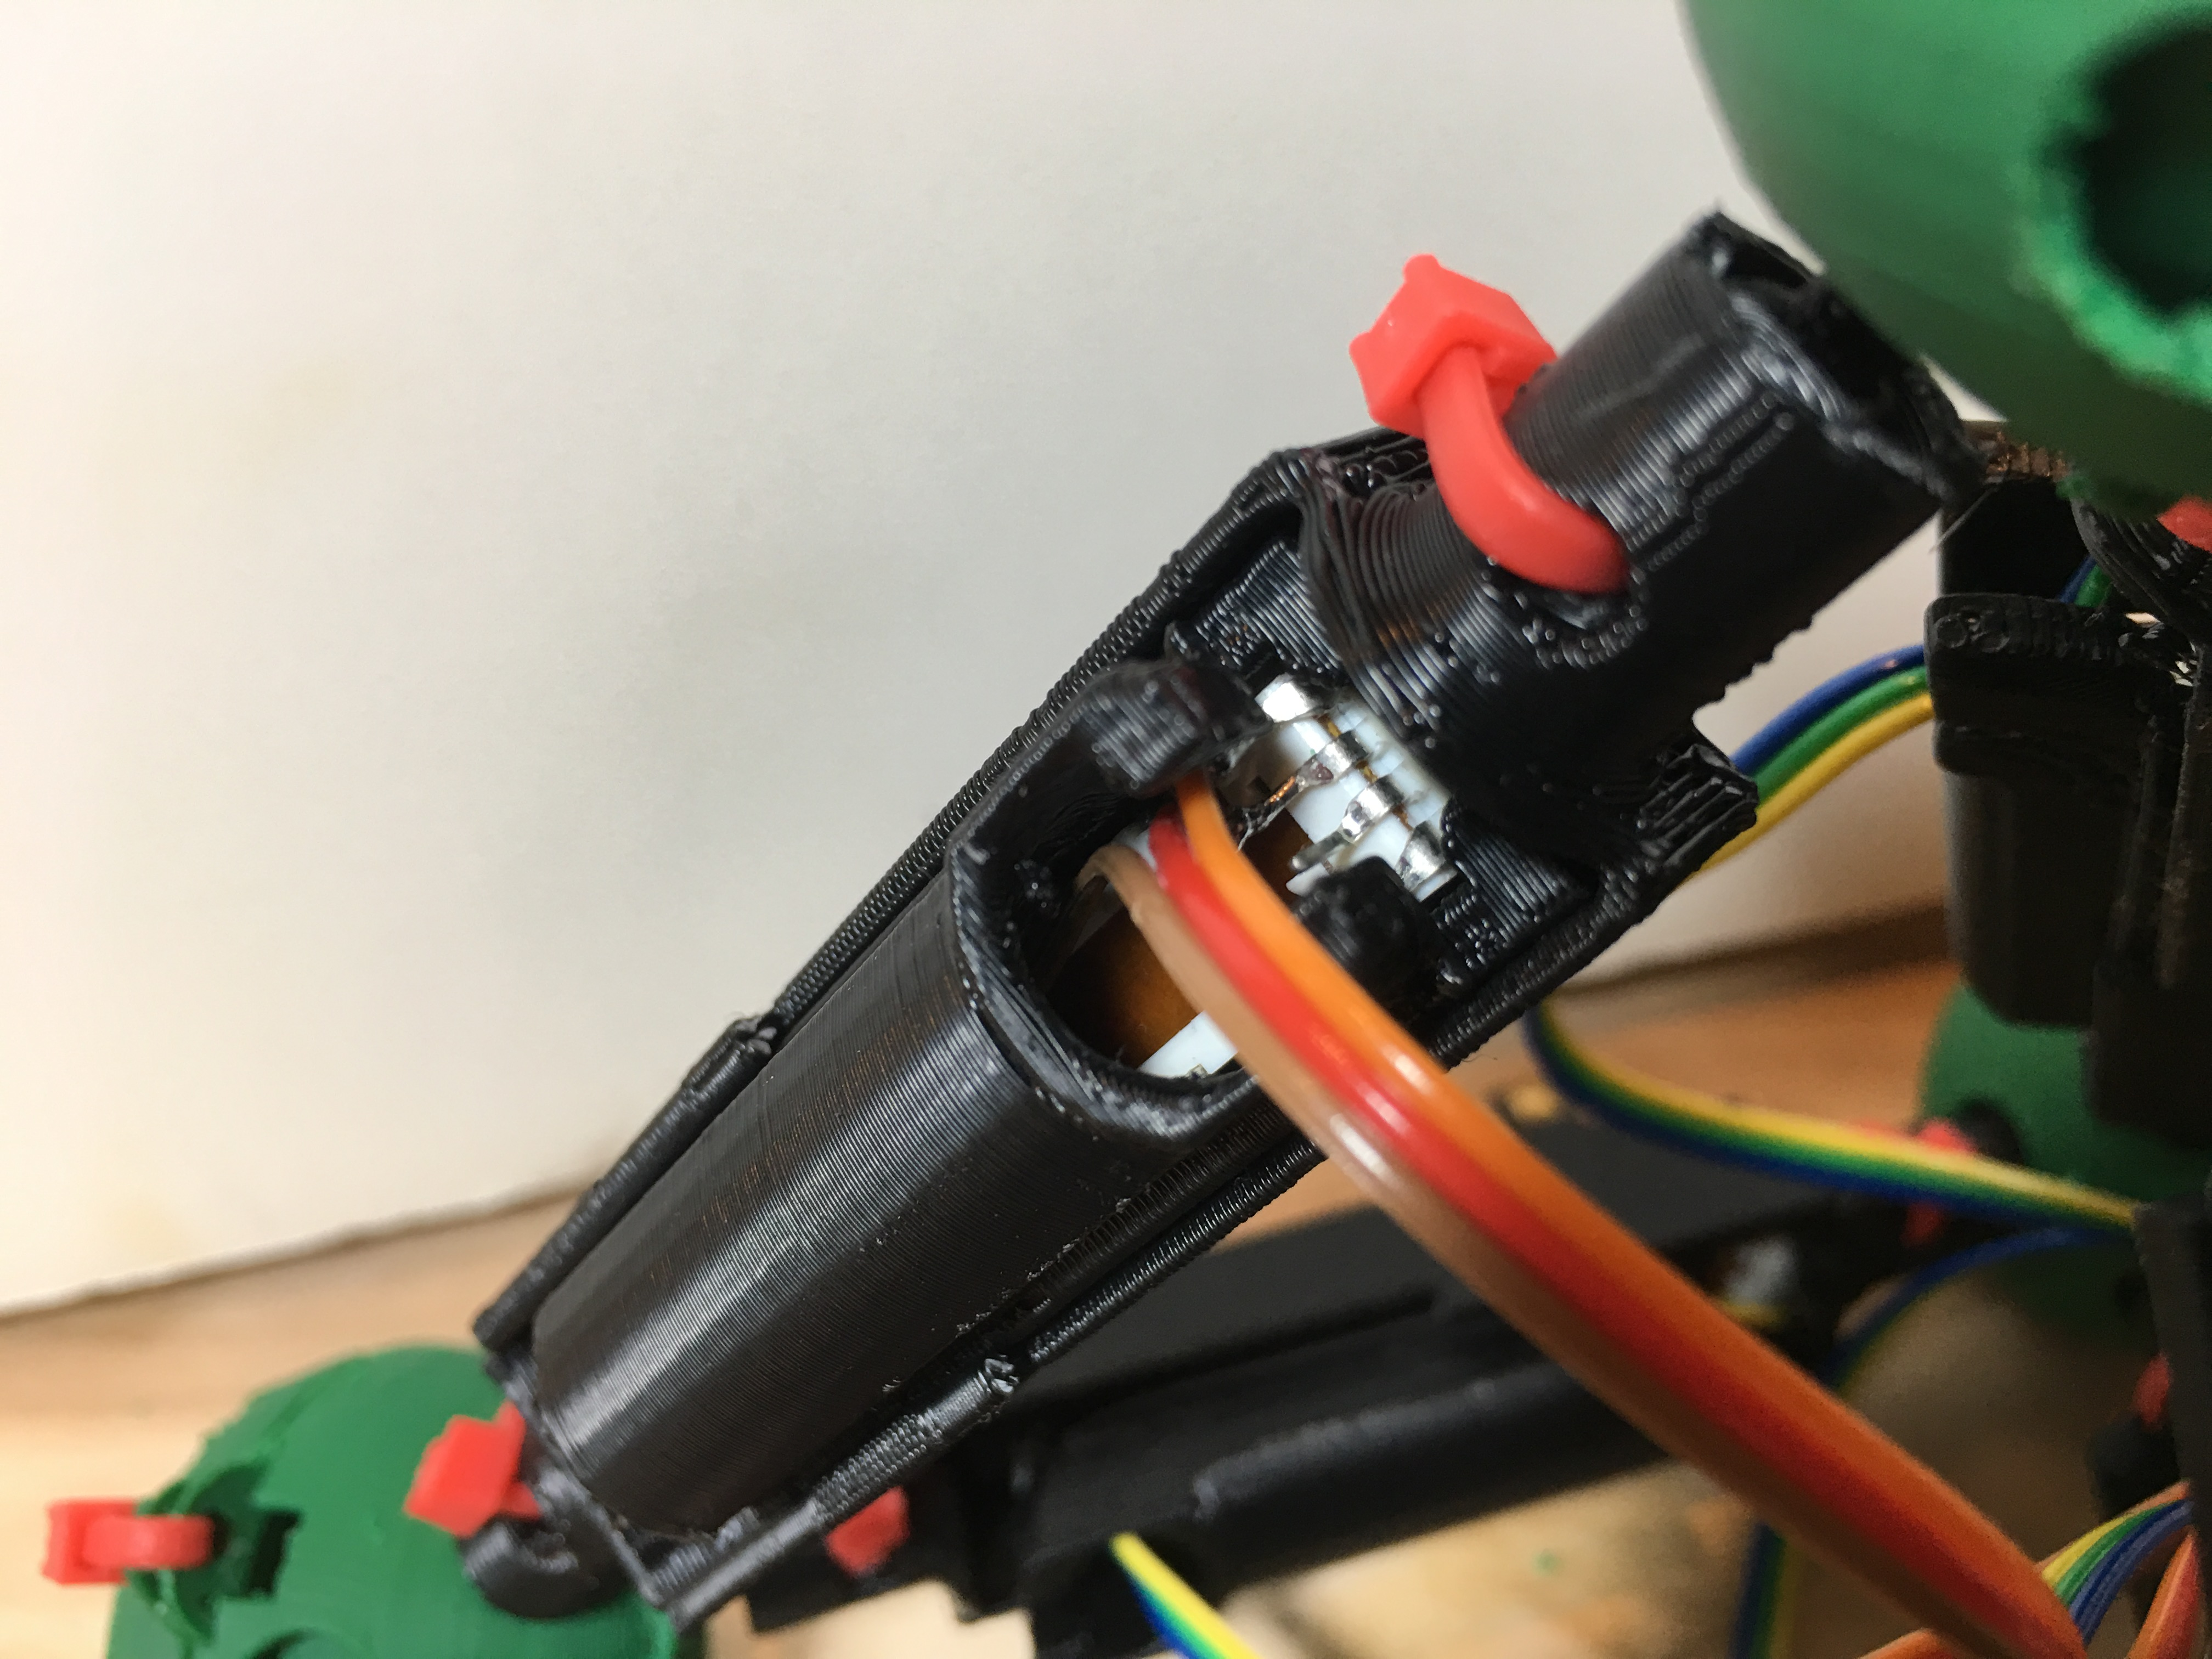
\includegraphics[width=0.5\textwidth]{figures/PotConnectionCloseUp.JPG}
    \caption[Close-up of Potentiometer Connection]{Close-up of Potentiometer Connection}
      \label{fig:potcloseup}
\end{figure}

\begin{figure}[H]
  \centering
    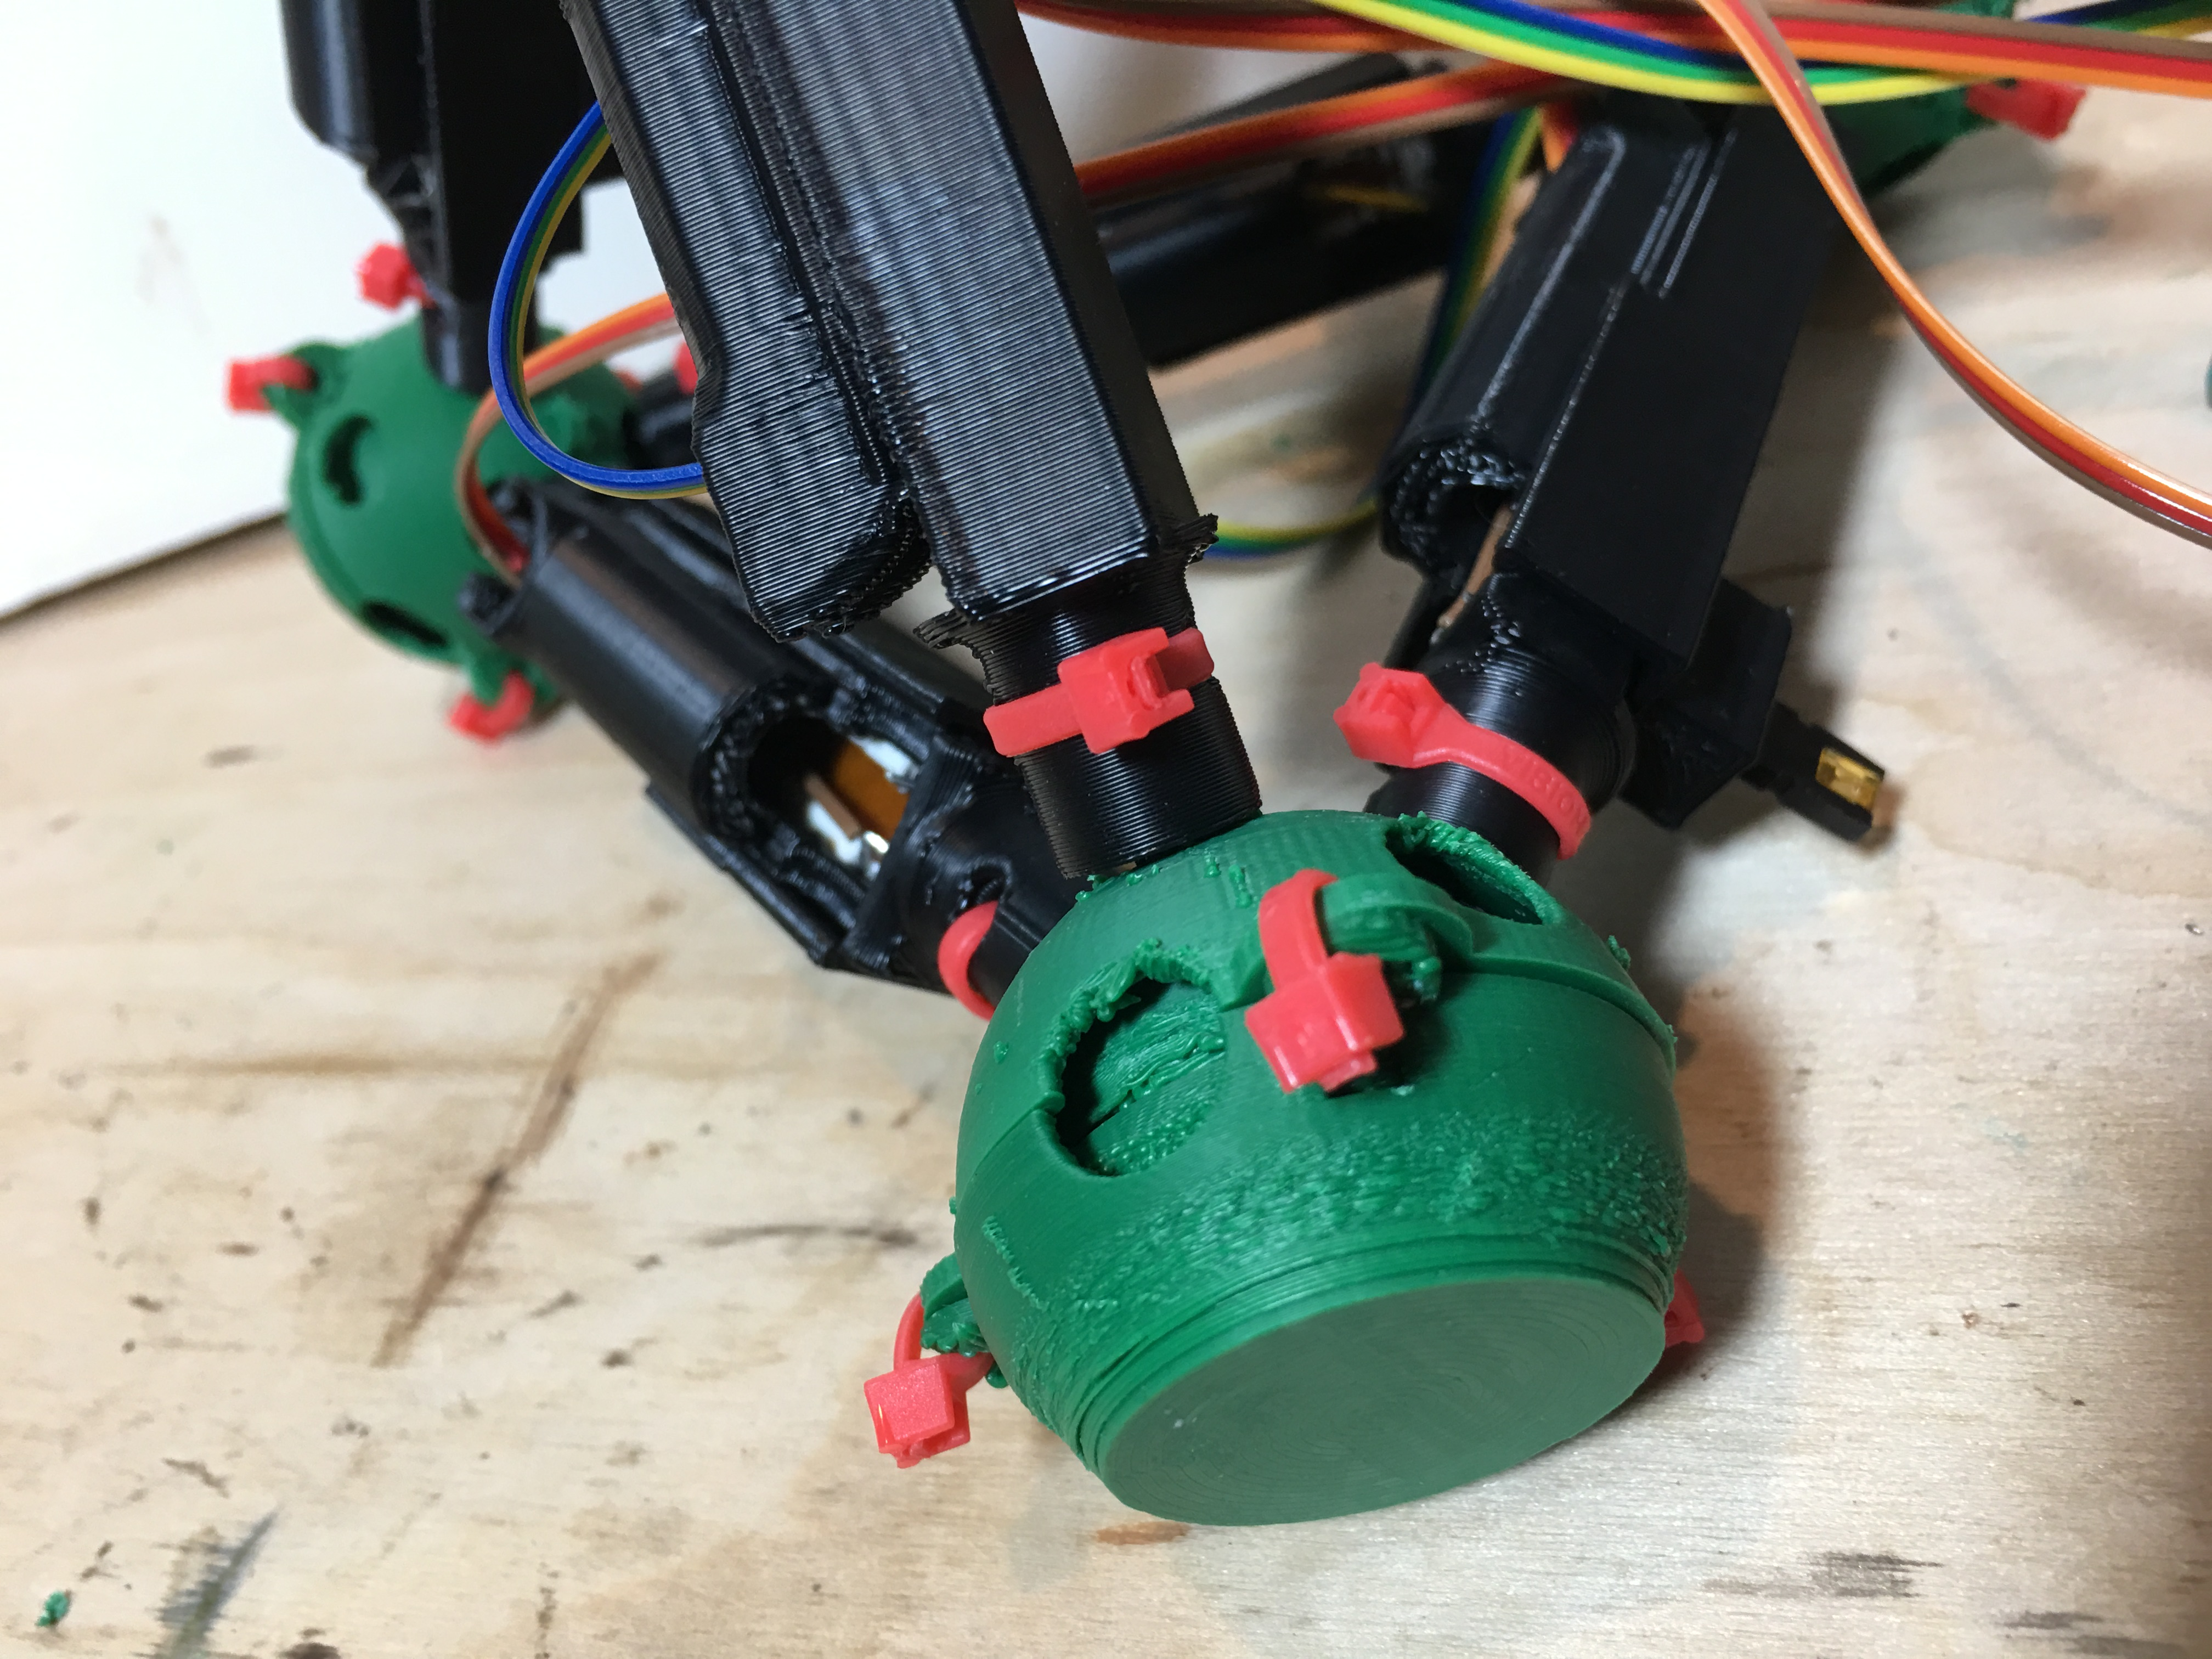
\includegraphics[width=0.5\textwidth]{figures/JointCloseUp.JPG}
    \caption[Joint Close Up]{Joint Close Up}
      \label{fig:jointcloseup}
\end{figure}

\begin{figure}[H]
  \centering
    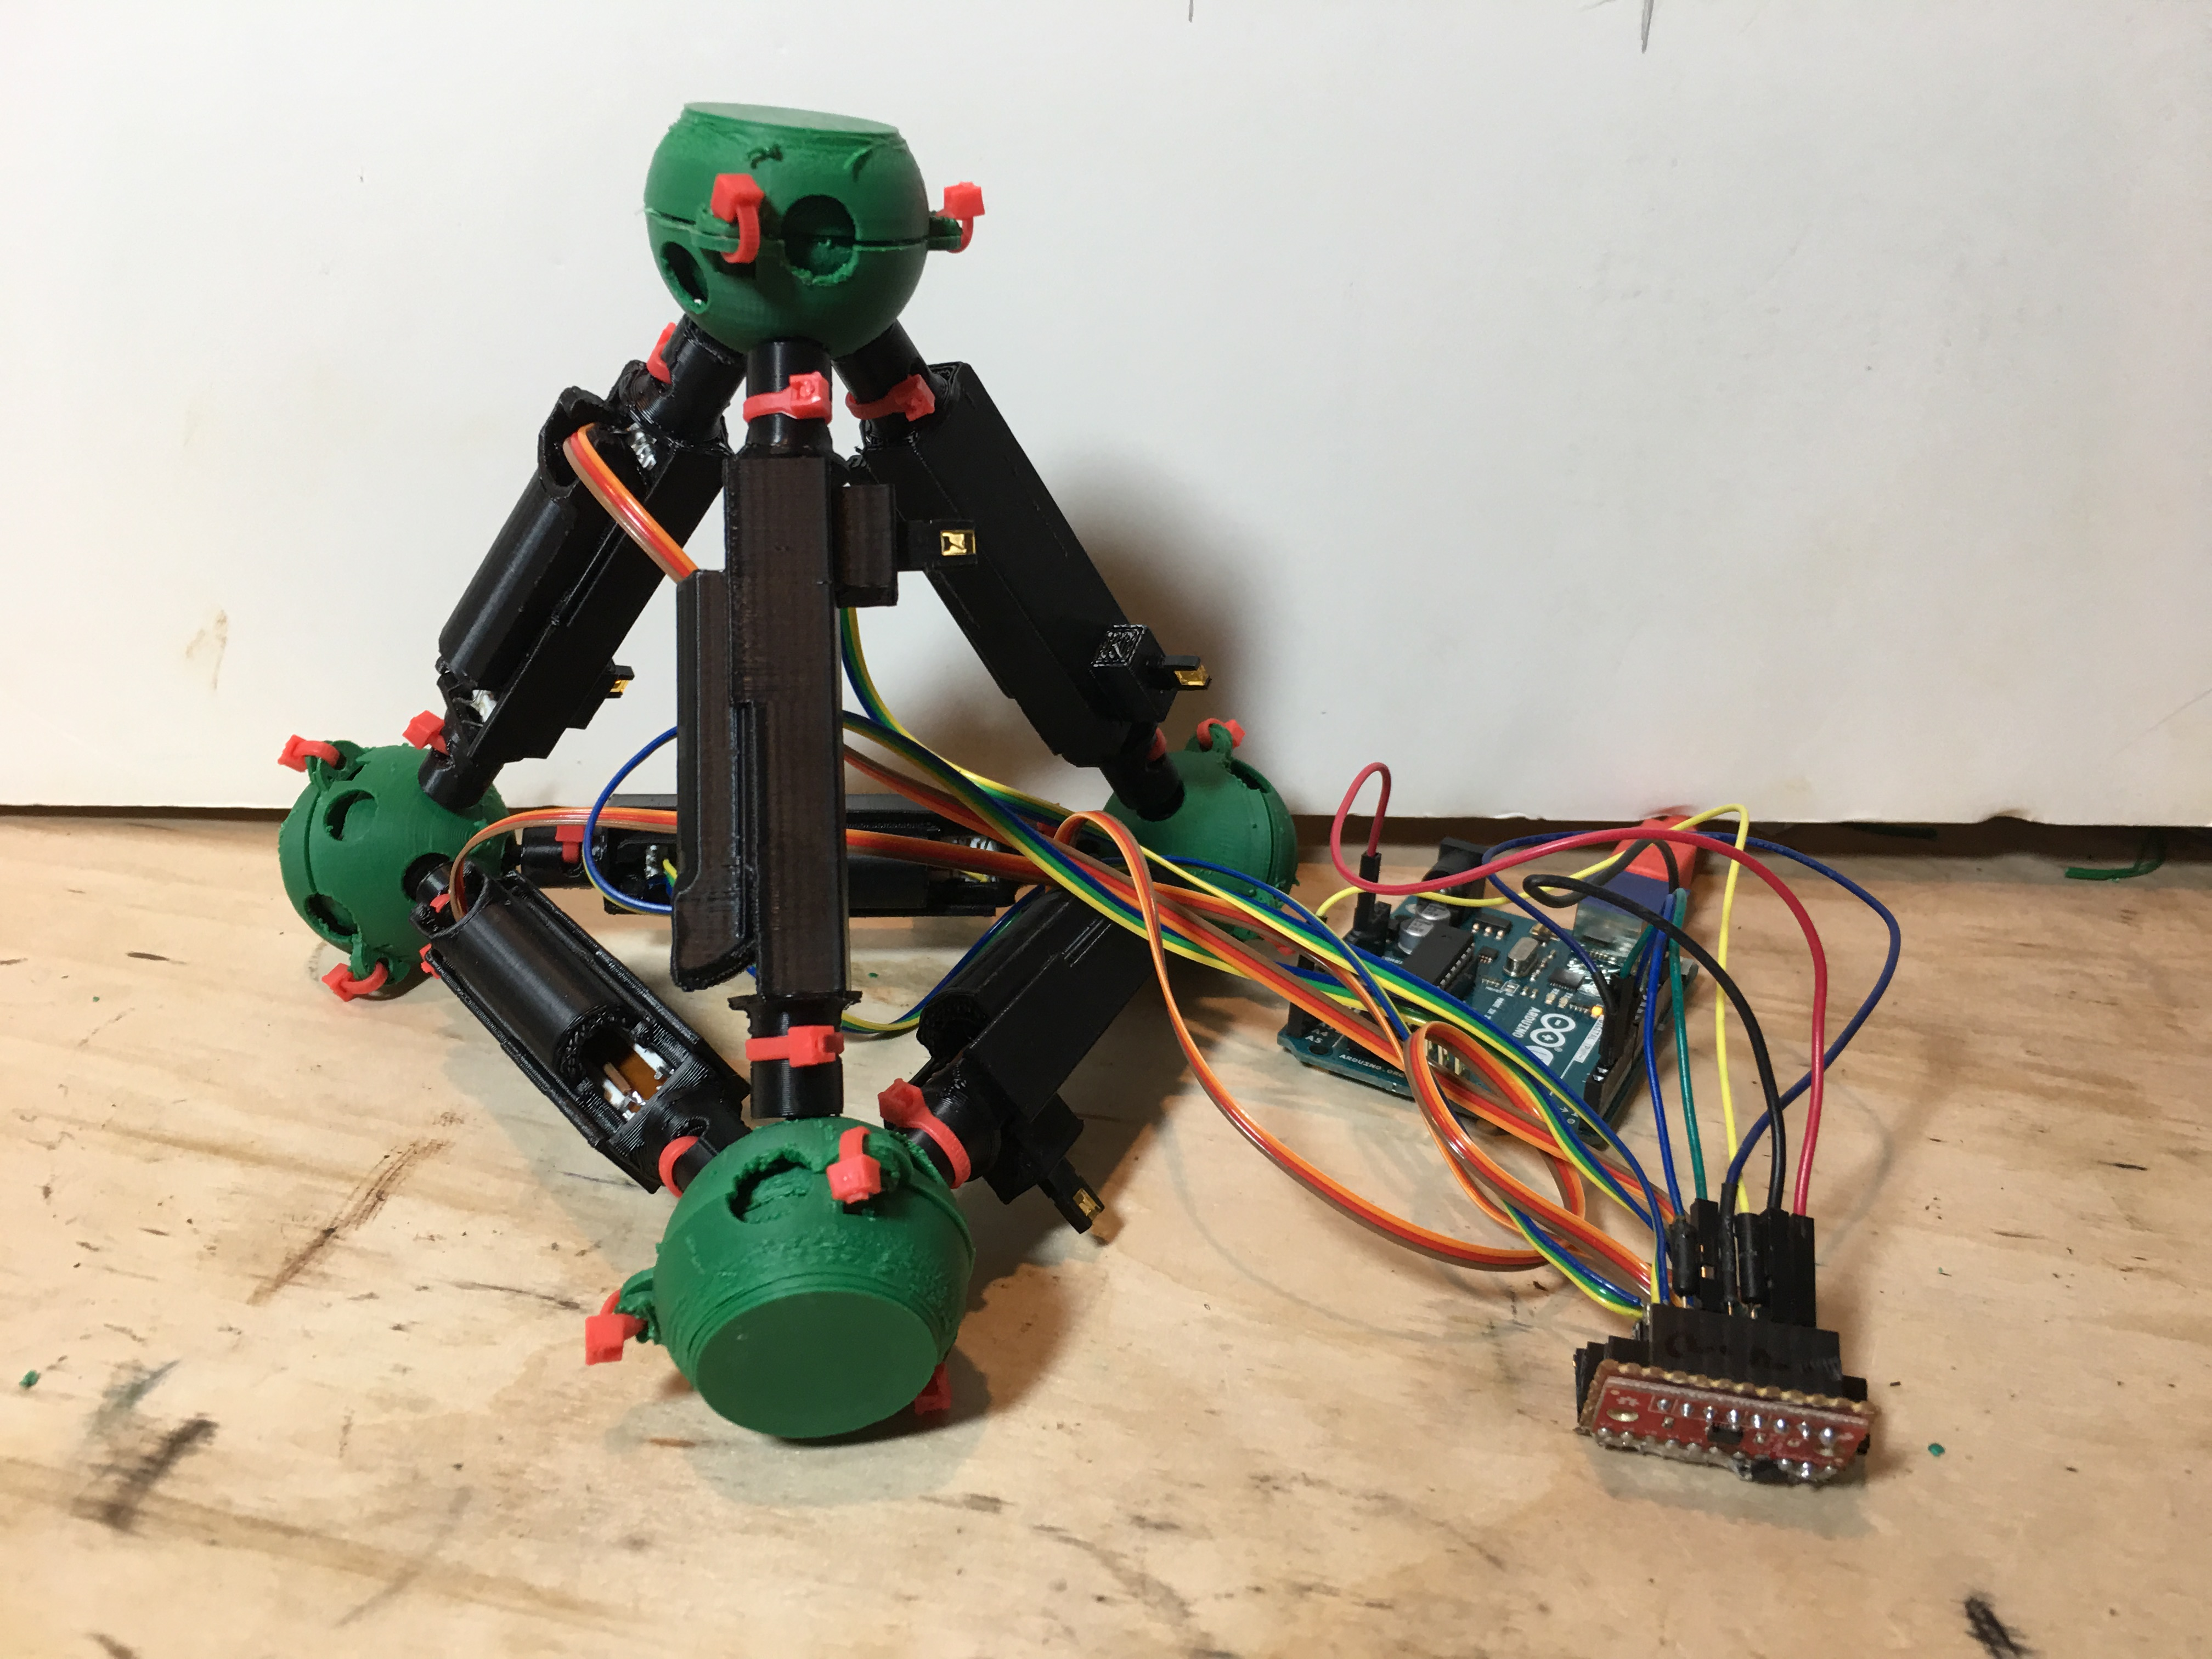
\includegraphics[width=0.5\textwidth]{figures/BasicOneTet.JPG}
    \caption[Basice One-Tet Controller]{Basic One-Tet Controller}
      \label{fig:basiconetet}
\end{figure}



\section{Future Steps}
\label{futuresteps}

\section{Contact and Getting Involved}

Public Invention
is a free-libre, open-source research, hardware, and software project that welcomes volunteers.
It is our goal to organize projects for the benefit of all humanity without seeking profit or intellectual property.
To assist, contact \href{mailto:read.robert@gmail.com}{$<$read.robert@gmail.com$>$}.

\bibliographystyle{plain}
\bibliography{gluss}

\end{document}
